\section{Branch Instructions}

\begin{concept}{Overview Branch Instructions}\\
Branch instructions control program flow:

\textcolor{darkcorn}{\textbf{Type:}}
\begin{itemize}
  \item \textbf{Unconditional:} Always taken
  \item \textbf{Conditional:} Branch if condition met
\end{itemize}

\textcolor{darktangerine}{\textbf{Address hand-over:}}
\begin{itemize}
  \item \textbf{Direct:} Target addresses part of instruction
  \item \textbf{Indirect:} Target address in register
\end{itemize}

\textcolor{darkfrog}{\textbf{Address of Target:}}
\begin{itemize}
  \item \textbf{Relative:} Target address relative to PC
  \item \textbf{Absolute:} Complete (absolute) target address
\end{itemize}

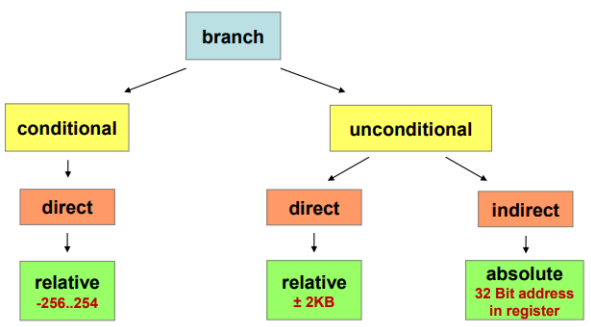
\includegraphics[width=\linewidth]{images/overview_branches.png}

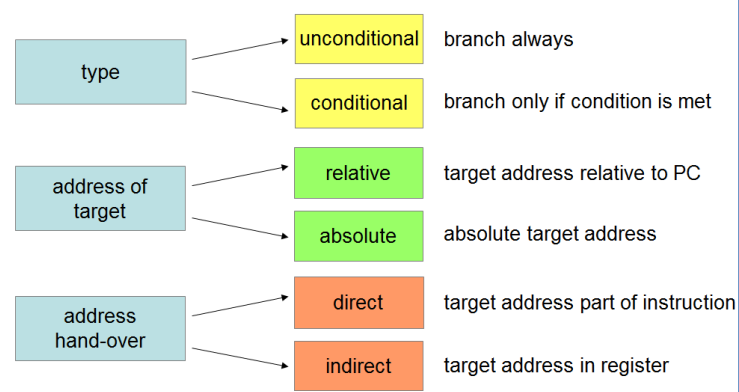
\includegraphics[width=\linewidth]{images/branchoverview2.png}
\end{concept}

\begin{corollary}{Types of Branches}\\
\textcolor{darkcorn}{\textbf{Unconditional}} Branches:
\begin{itemize}
    \item B (immediate)  $\rightarrow$ B label
    \begin{itemize}
        \item \textcolor{darktangerine}{\textbf{Direct}}
        \item \textcolor{darkfrog}{\textbf{Relative}}
    \end{itemize}
    \item BX (Branch and Exchange) $\rightarrow$ BX R0
    \begin{itemize}
        \item \textcolor{darktangerine}{\textbf{Indirect}}
        \item \textcolor{darkfrog}{\textbf{Absolute}}
    \end{itemize}
    \item BL (Branch with Link) $\rightarrow$ BL label
    \begin{itemize} 
        \item \textcolor{darktangerine}{\textbf{Indirect}}
        \item \textcolor{darkfrog}{\textbf{Absolute}}
    \end{itemize}
\end{itemize}

\textcolor{darkcorn}{\textbf{Conditional}} Branches:\\
Flag-dependent: BEQ, BNE, BCS, BCC, etc.\\
Arithmetic: BHI, BLS, BGE, BLT, etc.
\begin{itemize}
    \item \textcolor{darktangerine}{\textbf{Indirect}}
    \item \textcolor{darkfrog}{\textbf{Absolute}}
\end{itemize}
\end{corollary}



\begin{definition}{Flag dependant instructions}\\
Unsigned: Higher and Lower

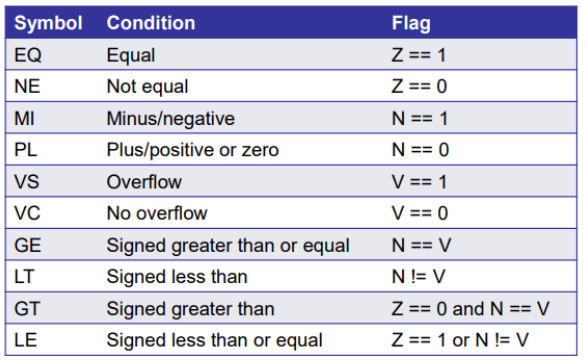
\includegraphics[width=\linewidth]{images/usnigned_flag_dependant_instruction.png}

Signed: Greater and Less

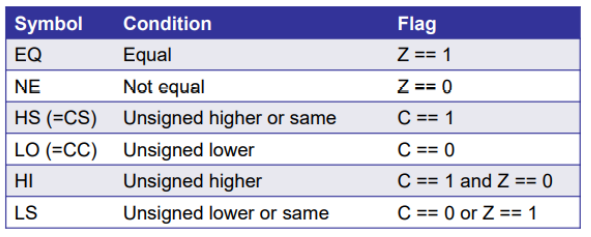
\includegraphics[width=\linewidth]{images/signed_flag_dependant_instruction.png}
\end{definition}

\begin{formula}{Compare and Test}
    \begin{itemize}
        \item TST: AND without changing the value
        \item CMP: SUB without changing the value
    \end{itemize}
\end{formula}

\begin{example2}{Comparison Instructions}
Using CMP and TST instructions:
\begin{lstlisting}[language=armasm, style=basesmol]
    ; Signed comparisons
    LDR     R1, =0xFFFFFFFF
    CMP     R1, #1          ; Compare with immediate
    BLT     is_less         ; Branch if less than
    
    ; Unsigned comparisons
    CMP     R1, #1
    BLO     is_below        ; Branch if lower
    
    ; Bit testing
    LDR     R5, =0x0040FFFF
    TST     R3, R5          ; Test bits
    BNE     bits_set        ; Branch if any bit set
    BEQ     bits_clear      ; Branch if all bits clear
\end{lstlisting}
\end{example2}

\begin{KR}{Branch Pattern Recognition}\\
Common branch patterns and their uses:

1. Basic branching:
\begin{lstlisting}[language=armasm, style=basesmol]
    ; Simple jump
    B       target          ; Unconditional
    BEQ     target          ; Branch if equal
    BNE     target          ; Branch if not equal
    
    ; Conditional execution
    CMP     R0, #value
    BCC     target          ; Branch if carry clear
    BGT     target          ; Branch if greater than
\end{lstlisting}

2. Jump tables:
\begin{lstlisting}[language=armasm, style=basesmol]
    ; Load table base
    LDR     R0, =jumptable
    ; Calculate offset
    LSLS    R1, R1, #2      ; Multiply index by 4
    ADDS    R0, R0, R1      ; Add to base
    ; Jump to handler
    LDR     R0, [R0]        ; Load address
    BX      R0              ; Branch to handler
\end{lstlisting}

3. Infinite loops:
\begin{lstlisting}[language=armasm, style=basesmol]
endless B       endless      ; Simple infinite loop

loop    ; Do something
        B       loop        ; Loop forever
\end{lstlisting}
\end{KR}

\begin{example2}{Conditional Branches with Flag Testing}\\
Example tracking non-taken branches:
\begin{lstlisting}[language=armasm, style=basesmol]
    MOVS    R0, #0          ; Clear mask
    
    ; Test carry flag
    ADDS    R1, R1, #5
    BCS     taken
    ADDS    R0, R0, #0x01   ; Mark if not taken
taken

    ; Test equality
    ANDS    R1, R1, R5
    BEQ     equal
    ADDS    R0, R0, #0x02   ; Mark if not taken
equal

    ; Test overflow
    SUBS    R2, R2, R5
    BVS     overflow
    ADDS    R0, R0, #0x04   ; Mark if not taken
overflow
\end{lstlisting}

Result in R0 shows which branches were not taken.
\end{example2}







